\documentclass{article}
\usepackage{tikz}
\begin{document}

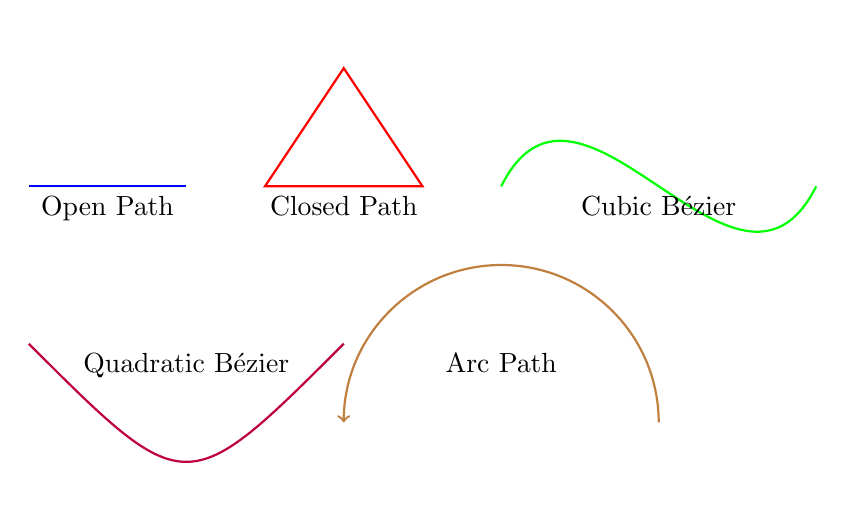
\begin{tikzpicture}[scale=1]

  % --- Open path ---
  \draw[blue, thick] (0,0) -- (2,0);
  \node[below] at (1,0) {Open Path};

  % --- Closed path ---
  \draw[red, thick] (3,0) -- (4,1.5) -- (5,0) -- cycle;
  \node[below] at (4,0) {Closed Path};

  % --- Cubic Bézier curve ---
  \draw[green, thick] (6,0) .. controls (7,2) and (9,-2) .. (10,0);
  \node[below] at (8,0) {Cubic Bézier};

  % --- Quadratic Bézier curve ---
  \draw[purple, thick] (0,-2) .. controls (2,-4) .. (4,-2);
  \node[below] at (2,-2) {Quadratic Bézier};

  % --- Arc path ---
  \draw[brown, thick, ->] (8,-3) arc(0:180:2);
  \node[below] at (6,-2) {Arc Path};

\end{tikzpicture}

\end{document}
